\documentclass{beamer}
\usetheme{Warsaw}
\useinnertheme{circles}
\useoutertheme[subsection=false]{smoothbars}
\usepackage[utf8x]{inputenc}
\usepackage[czech]{babel}
\usepackage[T1]{fontenc}
\usepackage{listings}
\usepackage{tikz}
\lstset{basicstyle=\tiny\ttfamily}
\logo{
\includegraphics[height=0.5cm]{brmlab.pdf}}

\begin{document}

\AtBeginSection[]
{
  \begin{frame}
    \frametitle{Outline}
    \tableofcontents[currentsection]
  \end{frame}
}

\title{brmiversity: Umělá inteligence \\ a teoretická informatika}
\subtitle{Přednáška č. 6}
\author{Petr Baudiš $\langle${\tt pasky@ucw.cz}$\rangle$}
\institute{
	brmlab 2011\\
	\vskip 1ex
	\pgfdeclareimage[height=4ex]{ccbysa}{by-sa.pdf}
	\pgfuseimage{ccbysa}
}
\date{}
\frame{\titlepage}

\section{Pravděpodobnost}

\subsection{}
\begin{frame}{Pravděpodobnost}
\begin{itemize}
\item Co je to
\item Dvě interpretace
\item Pozor na fuzzy logiku
\end{itemize}
\end{frame}

\subsection{}
\begin{frame}{Matematická pravděpodobnost}
\begin{itemize}
\item Operace s pravděpodobnostmi
\end{itemize}
\end{frame}

\subsection{}
\begin{frame}{Podmíněná pravděpodobnost}
\begin{itemize}
\item Podmíněná pravděpodobnost
\item Bayesovo pravidlo
\end{itemize}
\end{frame}

\subsection{}
\begin{frame}{Statistika}
\begin{itemize}
\item Měření pravděpodobnosti, střední hodnota, směrodatná odchylka a rozptyl
\end{itemize}
\end{frame}

\subsection{}
\begin{frame}{Pravděpodobnostní rozdělení}
\begin{itemize}
\item Pravděpodobnostní rozdělení
\end{itemize}
\end{frame}

\subsection{}
\begin{frame}{Normální rozdělení}
\begin{itemize}
\item Normální rozdělení, intervaly spolehlivosti
\end{itemize}
\end{frame}

\section{Umělá inteligence}

\subsection{}
\begin{frame}{Zpracování neurčité informace}
\begin{itemize}
\item Data o světě jsou neurčitá
\item Úkony ve světě jsou neurčitá
\item \dots takže reálný svět je neurčitý
\item Neurčitost: Usuzování, rozhodování, modelování, učení
\end{itemize}
\end{frame}

\subsection{}
\begin{frame}{Bayesovské sítě}
\begin{itemize}
\item Chceme modelovat svět provázaných náhodných jevů
\item Bayesovská síť: Graf (DAG), uzly jsou jevy, hrany jsou podmíněné vazby
\vskip 3ex
\item Co se stane, když vidím tohle?
\item Co bych měl zjistit, abych si co nejvíce upřesnil obraz o světě?
\item Na čem nejvíce závisí, že se tohle stane?
\item Kvůli čemu se asi stalo tohle?
\end{itemize}
\end{frame}

\subsection{}
\begin{frame}{Pravděpodobnostní rozhodovací stromy}
\begin{itemize}
\item Chceme posoudit dopady svých rozhodnutí \\
	Posloupnost rozhodnutí a neurčitých jevů vede k různému užitku
\item Rozhodovací stromy: Větvení na rozhodnutích a jevech, list je užitek
\item (Pozor, ``rozhodovací stromy'' se říká i něčemu jinému!)
\vskip 3ex
\item Kterou cestou má jet robot?
\end{itemize}
\end{frame}

\subsection{}
\begin{frame}{Influenční diagramy}
\begin{itemize}
\item Podstromy rozhodovacích stromů se často opakují, nezáleží na předchozích rozhodnutích a jevech
\item Influenční diagramy (rozhodovací grafy): Obecný graf, užitkové uzly udávají změnu užitku, když skrze ně projdeme
\end{itemize}
\end{frame}

\subsection{}
\begin{frame}{Otázky?}
\begin{center}
Příště UI: Modelování --- Markovské modely, Kalmanův filtr.
\end{center}
\end{frame}

\section{Složitost}

\subsection{}
\begin{frame}{Pravděpodobnostní algoritmy}
\begin{itemize}
\item Po algoritmu obvykle chceme, aby nám vrátil \\ přesný výsledek za přesný čas
\item Co když akceptujeme určitou {\em malou chybu}?
\item Co když akceptujeme, že {\em jen asi} doběhneme včas?
\vskip 3ex
\item Model: Probabilistický Turingův stroj
\end{itemize}
\end{frame}

\subsection{}
\begin{frame}{Monte Carlo}
\begin{columns}
\begin{column}{7cm}
\begin{itemize}
\item Monte Carlo algoritmus: \\ Čím déle běžíme, tím \\ přesnější výsledek dostaneme.
\item Třída složitosti BPP: Problém \\ řešitelný na probabilistickém TS \\ v polynomiálním čase \\ s pravděpodobností chyby $\le 1/3$
\vskip 3ex
\item Obsah průniku kružnic
\item Určitý integrál (plocha pod křivkou)
\item Prvočíselné testy
\item Monte Carlo Tree Search
\end{itemize}
\end{column}
\begin{column}{4cm}
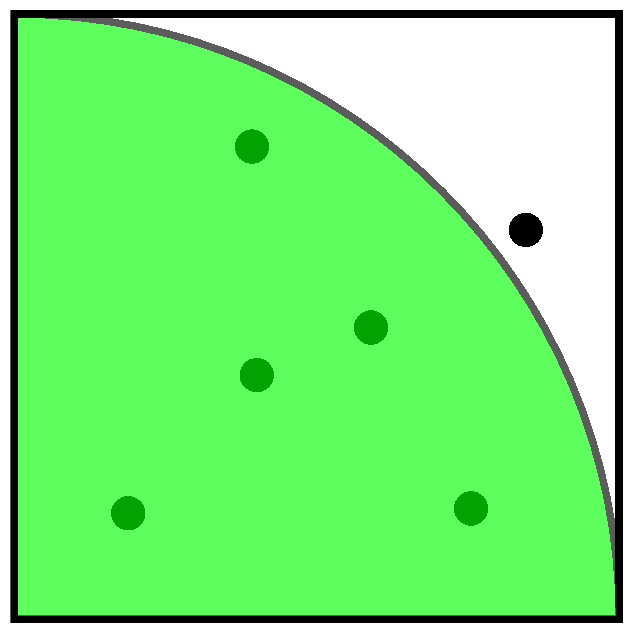
\includegraphics[width=4cm]{MC-pi.pdf}
\end{column}
\end{columns}
\end{frame}

\subsection{}
\begin{frame}{Las Vegas}
\begin{itemize}
\item Las Vegas algoritmus: {\em Očekávaná} doba běhu \\ je jiná než nejhorší
\item Třída složitosti ZPP: Problém řešitelný \\ na probabilistickém TS v očekávaném polynomiálním čase
\vskip 3ex
\item Quicksort s náhodnou volbou pivota
\vskip 3ex
\item Je Las Vegas a Monte Carlo ekvivalentní?
\end{itemize}
\end{frame}

\subsection{}
\begin{frame}{Otázky?}
\begin{center}
Příště: Míry složitosti, Savitchova věta, konstruovatelné funkce.
\end{center}
\end{frame}

\section{Datové struktury}

\subsection{}
\begin{frame}{Hashování}
\begin{itemize}
\item Hash tabulka (v paměti --- ``interní'').
\item Možná i nudle ven, řetězce.
\end{itemize}
\end{frame}

\subsection{}
\begin{frame}{Model hashování}
\begin{itemize}
\item Očekávaný počet kolizí, složitosti.
\end{itemize}
\end{frame}

\subsection{}
\begin{frame}{Externí hashování}
\begin{itemize}
\item Externí hashování.
\end{itemize}
\end{frame}

\subsection{}
\begin{frame}{Perfektní a univerzální hashování}
\begin{center}
Perfektní hashování: Chceme vyrobit read-only hash tabulku bez kolizí.

Univerzální hashování: Chceme vyrobit hashovací funkci odolnou k nerovnoměrnému rozdělení vstupu.
\end{center}
\end{frame}

\subsection{}
\begin{frame}{Otázky?}
\begin{center}
Příště: Univerzální a perfektní hashování. \\ A někdy doděláme ty haldy.
\end{center}
\end{frame}

\subsection{}
\begin{frame}{Děkuji vám}
\begin{center}
{\bf pasky@ucw.cz}

\vskip 6ex

Příště: Umělá inteligence. \\ Neuronové sítě (statistické zpracování dat). \\ Adaptivní agenti (komunikace a znalosti). Datové struktury.
\end{center}
\end{frame}

\end{document}
